% cpedoc.tex V2.0, 13 May 2010

\documentclass[times, doublespace]{cpeauth}

\usepackage{color}
\usepackage{listings}
\usepackage{multirow}
\usepackage{epstopdf}
\usepackage{graphicx}
\usepackage{algorithm}
\usepackage[caption=false]{subfig}
\usepackage{algorithm}
\usepackage[noend]{algpseudocode}
\usepackage{algpseudocode}
\algdef{SE}[FUNCTION]{Function}{EndFunction}
[2]{\algorithmicfunction\ \textproc{#1}\ifthenelse{\equal{#2}{}}{}{(#2)}}%
   {\algorithmicend\ \algorithmicfunction}%

\lstset{language=C,basicstyle=\small}
\lstset{numbers=left, numberstyle=\tiny, stepnumber=1, numbersep=5pt}
\lstset{tabsize=2}
\lstset{firstnumber=1}
\lstset{frame=single}
\lstset{
  language={C++},
  morekeywords={define,public,class,this,assert,exit,assume,then,end-if,end,input,output,true,false,bool,malloc,using,namespace,std,cudaError_t
		}
}

\hyphenation{
GKLEE 
property 
operational 
developed
ap-proxi-mates
pro-grams
inter-face
errors
par-ticu-lar
ver-ifiers
veri-fi-ca-tion
ori-gin-al
hier-archy
last-Error
in-de-pend-ent
pos-itions
array
ana-lysis
unsyn-chron-ized
values
total
ex-plor-ation
add-ition-al-ly
}

\usepackage{moreverb}
\usepackage[colorlinks,bookmarksopen,bookmarksnumbered,citecolor=red,urlcolor=red]{hyperref}

\newcommand\BibTeX{{\rmfamily B\kern-.05em \textsc{i\kern-.025em b}\kern-.08em
T\kern-.1667em\lower.7ex\hbox{E}\kern-.125emX}}

\def\volumeyear{2016}

\begin{document}

\runningheads{P.~A.~Pereira et al.}{SMT-Based Context-Bounded Model Checking for CUDA Programs}

\title{SMT-Based Context-Bounded Model Checking\\for CUDA Programs}

\author{P.~A.~Pereira\affil{1}, H.~F.~Albuquerque\affil{1}, I.~S.~da Silva\affil{1}, H.~M.~Marques\affil{1}, F.~R.~Monteiro\affil{1}, R.~dos S.~	Ferreira\affil{2}, and L.~C.~Cordeiro\affil{1}\corrauth}

\address{
\affilnum{1}Faculty of Technology, Federal University of Amazonas, Amazonas, Brazil\break
\affilnum{2}Department of Informatics, Federal University of Vi\c{c}osa, Minas Gerais, Brazil}

\corraddr{3000 Av. Rodrigo Ot{\'a}vio, 69077--000, Electronic and Information Research Center at Federal University of Amazonas, Manaus, Amazonas, Brazil.\\E-mail: lucascordeiro@ufam.edu.br}

\begin{abstract}
We present ESBMC-GPU tool, an extension to the Efficient SMT-Based Context-Bounded Model Checker (ESBMC), which is aimed at verifying Graphics Processing Unit (GPU) programs written for the Compute Unified Device Architecture (CUDA) platform. ESBMC-GPU uses an operational model, {\it i.e.}, an abstract representation of the standard CUDA libraries, which conservatively approximates their semantics, in order to verify CUDA-based programs. It then explicitly explores the possible interleavings (up to the given context bound), while treats each interleaving itself symbolically. Additionally, ESBMC-GPU employs the monotonic partial order reduction and the two-thread analysis to prune the state space exploration. Experimental results show that ESBMC-GPU can successfully verify $82\%$ of all benchmarks, while keeping lower rates of false results. Going further than previous attempts, ESBMC-GPU is able to detect more properties violations than other existing GPU verifiers due to its ability to verify errors of the program execution flow and to detect array out-of-bounds and data race violations.
\end{abstract}

\keywords{model checking; GPU; CUDA programs; formal verification;}

\maketitle

\vspace{-6pt}
%------------------------------
\section{Introduction}
\vspace{-2pt}
%------------------------------

{\bf C}ompute {\bf U}nified {\bf D}evice {\bf A}rchitecture (CUDA) is a parallel computing platform and {\bf A}pplication {\bf P}rogramming {\bf I}nterface (API) model created by NVIDIA~\cite{cuda:2012}, which extends C/C$++$ and Fortran, in order to create a computational model that aims to harness the computational power of {\bf G}raphical {\bf P}rocessing {\bf U}nits (GPUs)~\cite{gpu:2010}.\ As in other programming languages, errors in CUDA programs eventually occur, in particular, due to array out-of-bounds, arithmetic overflow, and division by zero violations.\ Additionally, since CUDA is a platform that deals with parallel programming, specific concurrency errors related to data race and barrier divergence can be exposed due to the non-deterministic behaviour of the threads interleavings~\cite{betts:2012}.

Here, we describe and evaluate an approach for verifying CUDA programs based on the {\bf E}fficient {\bf S}MT-Based Context-{\bf B}ounded {\bf M}odel {\bf C}hecker (ESBMC)~\cite{cordeiro:2011,cordeiro:2012,ramalho:2013}, named as ESBMC-GPU, using a CUDA operational model (COM), which is an abstract representation of the standard CUDA libraries ({\it i.e.}, the native API) that conservatively approximates their semantics. We describe the implementation of COM, its pre- and postconditions, and simulation features ({\it e.g.}, how elements are manipulated), and how these are applied to verify CUDA applications. In contrast to previous attempts~\cite{betts:2012,Li:2010,Li:2012,civl:2015}, we combine symbolic model checking, based on {\bf B}ounded {\bf M}odel {\bf C}hecking (BMC)~\cite{Biere:2009} and {\bf S}atisfiability {\bf M}odulo {\bf T}heories (SMT)~\cite{Barrett:2009} techniques, with explicit state-space exploration, similar to Cordeiro {\it et al.}~\cite{cordeiro:2011}. In particular, we explicitly explore the possible interleavings (up to the given context bound), while we treat each interleaving itself symbolically w.r.t. a given property.

To prune the state-space exploration, we apply {\bf M}onotonic {\bf P}artial {\bf O}rder {\bf R}eduction (MPOR)~\cite{KahlonWG09} to CUDA programs, which eliminates redundant interleavings without missing any behavior that can be exhibited by the program. We have modified the MPOR algorithm to identify transitions between threads that accessed different memory locations in the same array. Since CUDA kernels typically produce regular and independent access to explore the benefits of the GPU execution model, the application of MPOR routinely leads to substantial performance improvements in most benchmarks. Thus, using operational models that simulate CUDA libraries, together with MPOR implementation in ESBMC-GPU, we achieve significant (correct) results of CUDA kernels verification, primarily when compared to other state-of-the-art GPU verifiers~\cite{betts:2012,Li:2012,Li:2010,civl:2015}. Additionally, the present approach considers low-level aspects related to dynamic memory allocation, data transfer, memory deallocation, and overflow. Such violations are typically present in CUDA programs, however, they are routinely ignored by most GPU verifiers. Thus, we provide a more precise verification than other existing approaches, considering soundness of data passed by the main program to the kernel, with the drawback of leading to a higher verification time.

%---------------------------------
\subsection{Contributions}
\vspace{-2pt}
\label{sec:contributions}
%---------------------------------

We make four major contributions:
\vspace{-4pt}
\begin{itemize}
\item we extend benefits of SMT-based context-bounded model checking for CUDA programs, in the context of parallel programming for GPUs, to detect more failures than other existing approaches, while keeping lower rates of false results; although SMT-based context-bounded model checking is not a novel technique, we have not seen in the literature its application to verify CUDA programs.

\item this work marks the first application of MPOR to CUDA programs to identify array accesses, which are independent, leading to significant performance improvements.

\item we provide an effective and efficient tool implementation (ESBMC-GPU) to support the checking of several CUDA programs. ESBMC-GPU tool and all benchmarks used during the evaluation process are available at \url{http://esbmc-gpu.org}.

\item we provide an extensive experimental evaluation of our approach against GKLEE~\cite{Li:2012}, GPUVerify~\cite{betts:2012}, PUG~\cite{Li:2010}, and CIVL~\cite{civl:2015} using standard CUDA benchmarks, which are extracted from the literature~\cite{cuda:2012,betts:2012,cudaproguide:2015}. Experimental results also show that our present approach outperforms all existing GPU verifiers with respect to the number of correct results.
\end{itemize}


This paper extends our previous work~\cite{Pereira15,Pereira16}. The version of ESBMC-GPU described and evaluated here has been optimized and extended. It now expands our operational model to support more CUDA libraries ({\it e.g.}, math functions) and includes new SMT solvers as back-end for ESBMC-GPU ({\it e.g.}, Boolector, Yices, MathSAT, and CVC4). We also provide additional details about our operational model, the application of MPOR to CUDA programs, and the two-thread analysis. We have also significantly expanded the experimental basis, including a new GPU verifier (CIVL), and evaluate ESBMC-GPU with (respectively, compare it against) the most recent stable versions of the GPU verifiers. 

%---------------------------------
\subsection{Organization of this work}
\vspace{-2pt}
\label{sec:organization}
%---------------------------------

The remainder of the paper is organized as follows: In Section~\ref{sec:fundamentacao_teorica}, we first give a brief introduction to the CUDA programming language, existing verifiers for GPU, and the ESBMC verifier. In Section~\ref{sec:methodology}, we describe our operational models for CUDA libraries, the application of MPOR to CUDA programs, and our two-threads analysis. In Section~\ref{sec:resultadosExperimentais}, we present the results of our experiments using several publicly available benchmarks. In Section~\ref{sec:conclusions}, we conclude and describe future work.

%---------------------------------
\vspace{-6pt}
\section{Preliminaries}
\vspace{-2pt}
\label{sec:fundamentacao_teorica}
%---------------------------------

%---------------------------------
\subsection{CUDA Programming Language}
\vspace{-2pt}
\label{ssec:linguagem_cuda}
%---------------------------------

CUDA is a general-purpose parallel computing platform (developed by NVIDIA) to represent a programming model for GPUs~\cite{cuda:2012,cudaproguide:2015}. In the CUDA programming model, the kernel concept is used for a function that runs $n$ copies concurrently in the GPU, where $n$ is the product between the number of blocks and threads. A kernel is defined by a \emph{\tt \_\_global\_\_} specifier and uses the notation \emph{\tt kernel$<<<$ B,T $>>>$}, where $B$ and $T$ are the number of blocks and threads per block, respectively. Each kernel runs in the GPU as thread and each thread receives an unique identifier (ID), which is formed by thread and block numbers. The thread ID is used to index its tasks ({\it i.e.}, memory positions and cooperation); and threads are typically organized by blocks in the GPU.
Inside a block, the thread hierarchy is defined by a variable called \emph{\tt threadIdx}. This variable is a vector of three components, which allows the use of uni-, two-, and three-dimensional indexes~\cite{cudaproguide:2015}. 

Blocks can also be defined in three dimensions, where each dimension can be accessed by the \emph{\tt blockIdx} variable. This variable is also composed by three components that allow CUDA programs to use uni-, two-, and three-dimensional blocks.
The maximum number of threads per block depends on the hardware platform, but it usually ranges from $1024$ to $2048$~\cite{cudaproguide:2015}. In addition, blocks have a feature that permits them to be executed in any order; and they can also be allocated in any processor. As a result, a kernel may also be executed by multiple blocks, and the total number of threads represents the number of blocks multiplied by the number of threads per block.

In the CUDA programming model, the GPU is refereed as a \textit{device} and the \textbf{C}entral \textbf{P}rocessing \textbf{U}nit (CPU) is refereed as a \textit{host}. $\_\_device\_\_$ is a specifier for functions, which are executed and called only by the GPU, while $\_\_host\_\_$ is a specifier for functions, which are executed and called only by the CPU. $\_\_global\_\_$ is a function specifier that operates as an entry point for executing the kernels. The data allocation in the \textit{device} is carried out by the \textit{host}, using the \textit{cudaMalloc}, \textit{cudaFree}, and \textit{cudaMemcpy} functions. Importantly, these are essential functions for CUDA programs, to transfer data from the \textit{host} to the \textit{device} and vice-versa. 

%---------------------------------
\subsection{Existing GPU Verifiers}
\vspace{-2pt}
\label{ssec:trabalhos_relacionados}
%---------------------------------

GPUVerify~\cite{betts:2012} proposes a new operational semantics, known as \textbf{S}ynchronous \textbf{D}elayed \textbf{V}isibility (SDV) semantics to verify kernels, which aims to detect data race and barrier divergence. It uses the Boogie verification system~\cite{boogie:2011} to generate verification conditions, which are solved by Z3~\cite{Moura:2008} or CVC4~\cite{CVC4Barrett11} SMT solvers. GPUVerify accepts only kernel function as input, and it disregards the main function, which thus exposes incorrect results for verifying low-level aspects of CUDA programs.

\textbf{S}ymbolic \textbf{E}xecutor with \textbf{S}tatic \textbf{A}nalysis (SESA)~\cite{sesa:2014} and GPU + KLEE (GKLEE)~\cite{Li:2012} are verifiers based on the \textit{concolic} (concrete, but symbolic) execution of CUDA programs; nevertheless they use different approaches to determine symbolic variables. While SESA performs an automatic evaluation, GKLEE needs inputs from the user to define those variables. On the one hand, SESA checks real applications using original configuration of the number of threads and its focus is on data race detection, but it presents inconclusive results regarding access to memory positions.\ On the other hand, GKLEE supports checks related to barrier synchronization, functional correctness, performance, and data race. Importantly, SESA does not verify the main function, while GKLEE considers both kernel and main functions.

\textbf{P}rover of \textbf{U}ser \textbf{G}PU Programs (PUG)~\cite{Li:2010} analyzes kernels automatically using SMT solvers and it detects data race, barrier synchronization, and conflicts on shared memory. PUG faces problems with invariant derivation for loops, which can lead to incorrect results, and thus requires the user to provide those invariants.\ In addition, problems are also found in arithmetic operations of pointers and advanced C$++$ features.

CIVL~\cite{civl:2015} is a framework for static analysis and concurrent program verification, which supports MPI, POSIX, OpenMP, and CUDA. CIVL recognizes programs written in C++$11$, CUDA--C, and CIVL--C, which is an intermediate language that represents ANSI-C programs based on the aforementioned libraries. CIVL is the tool that is closer to ESBMC-GPU in terms of verification techniques, verifying the concurrent program with partial order reduction, in order to eliminate unnecessary interleavings. The verified properties include: user-specified assertions, deadlocks, memory leaks, invalid pointer dereference, array out-of-bounds, and division by zero. The support of CIVL for CUDA libraries is still in progress, being effective and efficient in programs with kernels that do not use many CUDA functionalities.

%---------------------------------
\subsection{ESBMC}
\vspace{-2pt}
\label{ssec:esbmc}
%---------------------------------

ESBMC is an open source, permissively licensed, award-winning context-bounded model checker for C/C$++$ programs based on SMT solvers~\cite{cordeiro:2011,cordeiro:2012,Morse11,Morse:15}. It is able to verify single- and multi-threaded software with shared variables and locks using the Phtread/POSIX. In particular, ESBMC is one of the most prominent BMC tools for verifying ANSI-C programs according to the last editions of the International \textbf{Comp}etition on \textbf{S}oftware \textbf{V}erification (SV-COMP)~\cite{svcomp2014,svcomp2015}. ESBMC can verify programs that contain bit-level, arrays, structs/unions, pointers, dynamic memory allocation, as well as fixed-point arithmetic. It can reason about arithmetic overflows, pointer safety, memory leaks, array out-of-bounds, atomicity and order violations, local and global deadlocks, data races, and user-specified assertions.

In ESBMC, ANSI-C/C++ programs are typically represented as a state transition system $M = (S, R, s_{0})$, which are extracted from the \textbf{C}ontrol-\textbf{F}low \textbf{G}raph (CFG). $S$ represents the set of states, $R \subseteq S \times S$ represents the set of transitions, and $s_{0} \subseteq S$ represents the set of initial states.\ A state $s \in S$ consists of the value  of the program counter \emph{pc} and the values of all program variables.\ An initial state $s_{0}$ assigns the initial program location of the CFG to \emph{pc}.\ Each transition $\gamma=(s_i,s_{i+1}) \in R$ between two states $s_{i}$ and $s_{i+1}$ is identified with a logical formula $\gamma(s_i,s_{i+1})$, which captures constraints on the corresponding values of the program counter and the program variables.

In particular, consider the transition system \textit{M}, a safety property $\phi$, a context bound $C$, and a bound $k$, ESBMC constructs a \textbf{R}eachability \textbf{T}ree (RT), which represents the program unfolding for $C$, $k$, and $\phi$. A \textbf{v}erification \textbf{c}ondition (VC) $\psi^{\pi}_{k}$ is then derived for each given interleaving $\pi = \{\nu_1,\ldots, \nu_k\}$, such that $\psi^{\pi}_{k}$ is satisfiable \textit{iff} $\phi$ has a counterexample of depth \textit{k}, which is exhibited by $\pi$.\ $\psi^{\pi}_{k}$ is given as follows
%
\begin{equation} \label{bounded-model-checking} \psi^{\pi}_{k} =
I(s_{0}) 
\wedge 
  \bigvee^{k}_{i=0} \bigwedge^{i-1}_{j=0} \gamma(s_{j},s_{j+1})
\wedge 
  \neg \phi(s_i)
\end{equation}
%
\noindent $I$ characterizes the set of initial states of $M$ and $\gamma(s_{j},s_{j+1})$ is the transition relation of $M$ between time steps $j$ and $j+1$. Hence, $I(s_0)\wedge\bigwedge^{i-1}_{j=0} \gamma(s_{j},s_{j+1})$ represents executions of $M$ of length $i$ and $\psi^{\pi}_{k}$ can be satisfied if and only if for some $i \leq k$ there exists a reachable state along $\pi$ at time step $i$ in which $\phi$ is violated. $\psi^{\pi}_{k}$ is a quantifier-free formula in a decidable subset of first-order logic, which is checked for satisfiability by an SMT solver. If $\psi^{\pi}_{k}$ is satisfiable, then $\phi$ is violated along $\pi$ and the SMT solver provides a satisfying assignment, from which the  program variables values can be extracted, in order to construct a counterexample. A counterexample for a particular property $\phi$ is a sequence of states $s_{0}, s_{1},\ldots, s_{k}$ with $s_{0} \in S_{0}$, $s_{k} \in S$, and $\gamma\left(s_{i}, s_{i+1}\right)$ for $0 \leq i < k$. If $\psi^{\pi}_{k}$ is unsatisfiable, one can conclude that no error state is reachable in $k$ steps or less along $\pi$. Finally, we can define $\psi_{k} = \bigwedge_{\pi}\psi^{\pi}_{k}$ and use this to check all paths. 

ESBMC combines symbolic model checking with explicit state space exploration; in particular, it explicitly explores the possible interleavings (up to the given context bound) while it treats each interleaving itself symbolically. ESBMC simply traverses the RT depth-first, and calls the single-threaded BMC procedure on the interleaving whenever it reaches an RT leaf node. It stops when it finds a bug, or has systematically explored all possible RT interleavings.

%---------------------------------
\subsubsection{Software Architecture}
\vspace{-2pt}
\label{ssec:SoftwareArchitecture}
%---------------------------------

\begin{figure*}[htb]
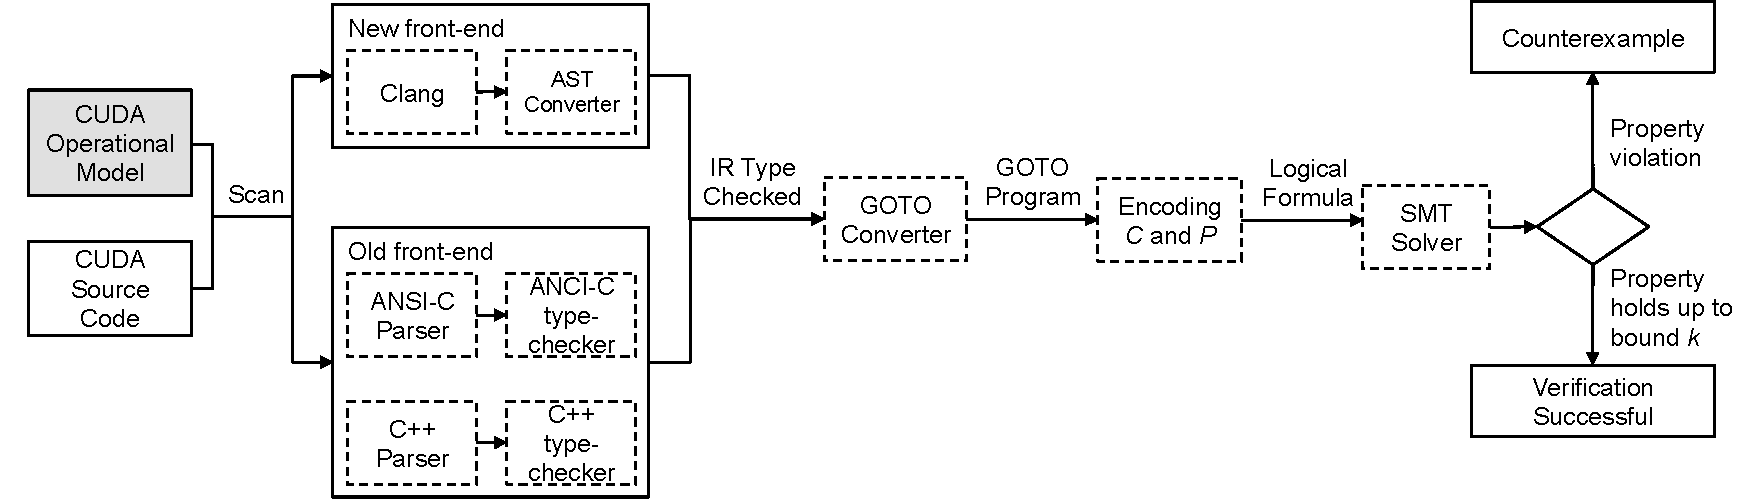
\includegraphics[width=\textwidth]{images/esbmc-arch-2}
\caption{ESBMC architecture.}
\label{figure:esbmc-arch}
\end{figure*}

Fig.~\ref{figure:esbmc-arch} shows the ESBMC architecture. Rounded white
rectangles represent input and output; Squared gray rectangles represent the
verification steps.

ESBMC offers two front-ends to parse and generate the \textbf{I}ntermediate
\textbf{R}epresentation (IR) of the program. On the old front-end, based on
one from CBMC~\cite{Clarke:2004}, ESBMC would first
parse the program using flex/bison~\cite{Levine:2009:FB:1696439} to generate an
\textbf{A}bstract \textbf{S}yntax \textbf{T}ree (AST), which is converted to IR. The IR is then type-checked,
which is language-specific. During the type-checking, the code is statically
analysed, including assignment checks, type-cast checks, pointer
initialisation checks, function call checks and template instantiation.

The new front-end offers a much simpler and stronger alternative, but it does not support C++ yet. 
In particular, the new front-end uses clang~\cite{Lopes:2014:GSL:2692607} to generate an AST, which is
then converted to an IR. Clang is a state-of-art compiler for
C/C++/ObjectiveC/ObjectiveC++ that it is already heavily used in
industry~\cite{clang-usage}. The compiler offers an industry level static
analyser and an API to access and traverse its internal AST, which is used by
ESBMC to generate its IR. By using clang, we avoid the need to maintain our own
front-end (a real challenge, given that the ANSI-C and C++ standards are rapidly
evolving nowadays), and can focus on the main objective of the tool, the formal
verification of a program. ESBMC currently can only convert the AST generated
for ANSI-C programs.

The subsequent steps are the same as already described us in previous
papers~\cite{cordeiro:2012}. Regardless of the chosen front-end, the output is the
IR that will be used by the GOTO converter to generate the GOTO program, which
is a simplified version of the original program. The symbolic execution executes
the GOTO program (unrolling loops up to bound \emph{k}) and converts the
expressions to \textbf{S}tatic \textbf{S}ingle \textbf{A}ssignments (SSA)~\cite{cytron89}. Finally, two
sets of quantifier-free formula are created based on the SSA expressions
(\textit{C} for the constraints and \textit{P} for the properties), and used as
input for an SMT solver that will produce a counterexample if there is a
violation of a given property, or an unsatisfiable answer (\textit{i.e.}, verification
successful) if the property holds.

%----------------------------------------------	    	
\vspace{-6pt}
\section{Verifying CUDA Programs}
\label{sec:methodology}
\vspace{-2pt}
\label{sec:metodologiaProposta}
%----------------------------------------------

%----------------------------------------------
\subsection{Operational Models for CUDA Libraries}
\vspace{-2pt}
\label{sec:modeloOperacional}
%----------------------------------------------

In order to correctly support CUDA functionalities, operational models are developed to reliably simulate the behavior of the CUDA libraries. Such approach was previously attempted in the formal verification of C++ programs~\cite{ramalho:2013}, Qt-based applications~\cite{monteiro:2015,garcia:2016}, and Android mobile applications~\cite{android:2012,android:2015}. In particular, our operational model consists of an abstract representation of a set of methods and data structures, which conservatively approximate the CUDA libraries semantics; every method simulates the library's real behavior, including pre- and post-conditions by means of assertions to ensure the correct operation.\ Thus, the operational model contains only methods for verification, ignoring irrelevant calls ({\it e.g.}, screen-printing methods), where there is no relevant property to be checked in terms of software. As a result, our verification focuses on the operational model of the CUDA libraries, and how it is used to verify real-world CUDA programs; this simplifies significantly the model verification and consequently reduces the verification time. The operational model also includes built-in assertions, which check specific properties ({\it e.g.}, array out-of-bounds, arithmetic overflow, pointer safety, and data races). As shown in Fig.~\ref{figure:com}, the operational model is passed to ESBMC's front-end together with the source code to be verified, in order to produce reliable AST with all relevant information for a trustful verification process.

\begin{figure*}[htb]
\centering
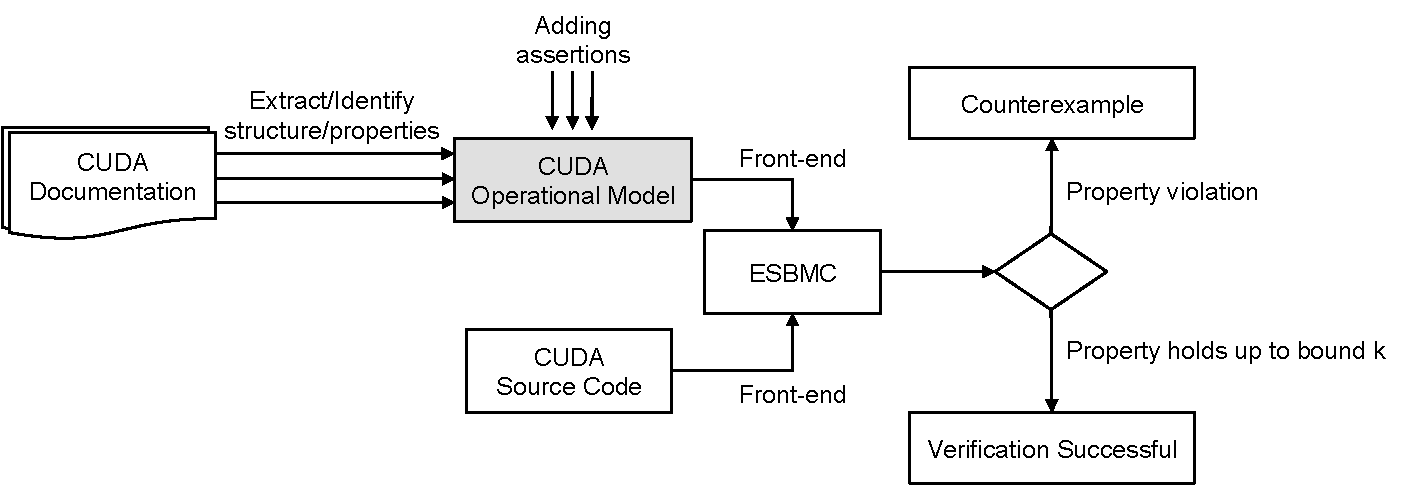
\includegraphics[width=120mm]{images/cuda-operational-model.pdf}
\caption{Link between CUDA operational model and ESBMC.}
\label{figure:com}
\end{figure*}

In our CUDA operational model (COM), methods, data types, qualifiers, and CUDA directives were implemented in C$++$. As an example, Figure~\ref{fig:dim3_implementation} shows the implementation of the data type \emph{\tt dim3}, which is represented by a \emph{\tt struct} with three variables: $x$, $y$, and $z$. The \emph{\tt dim3} model has a default constructor, a constructor that receives a variable \emph{\tt uint3} as parameter (this variable is modelled by a \emph{\tt struct} with three \emph{\tt uint} variables), and a constructor that is initialized by a \emph{\tt dim3} variable. In addition to the (typical) primitive data types of ANSI-C/C$++$, COM supports specific data types of CUDA (\textit{e.g.}, \emph{\tt char1}, \emph{\tt short2}, and \emph{\tt float2}).

\begin{figure} [htb]
\centering
\begin{minipage}{0.95\textwidth}
\begin{lstlisting}
struct __dim3
{
  unsigned int x, y, z;
  __dim3(unsigned int vx=1, unsigned int vy=1, unsigned int vz=1){
  	x=vx; y=vy; z=vz;
  }
  __dim3(uint3 v){
  	x=v.x; y=v.y; z=v.z;
  }
  __dim3(__dim3 d){
  	x=d.x; y=d.y; z=d.z;
  }
  operator uint3(void){
  	uint3 t; t.x=x; t.y=y; t.z=z;
	return t;
  }
};
typedef struct __dim3 dim3;
\end{lstlisting}
\end{minipage}
\caption{\emph{\tt dim3} implementation.}
\label{fig:dim3_implementation}
\end{figure}

COM also models methods typically used to develop real CUDA applications. In this sense, we support most CUDA driver and runtime APIs; in particular, ESBMC-GPU supports the CUDA call kernel (\textit{device\_launch\_parameters} and \textit{vector\_types}), driver\_types (\textit{math\_functions}, \textit{cuda\_runtime\_api}, and \textit{host\_definitions}), sm\_atomic\_functions (\textit{vector\_types}), and curand\_kernel (\textit{curand}). Figure~\ref{figure:comOrganization} shows the CUDA operational model organization (internally) implemented in ESBMC-GPU.

\begin{figure*}[htb]
\centering
\includegraphics[width=130mm]{images/com.pdf}
\caption{CUDA Operational Model Organization.}
\label{figure:comOrganization}
\end{figure*}

Here, we describe three essential functions in CUDA programs: \textit{cudaMalloc}, \textit{cudaMemcpy}, and \textit{cudaFree}. Algorithm~\ref{cudaMalloc-algorithm} shows an example of an operational model developed for the \textit{cudaMalloc} function, which abstracts the GPU memory hierarchy and accepts as input arguments, a pointer to allocate memory on the device ({\it i.e.}, \textit{devPtr}) and the size in \textit{bytes} needed for memory allocation (\textit{i.e.}, $size$). In order to allocate memory for \textit{devPtr} pointer (in step $3$), this algorithm uses the \textit{malloc} function, which represents the memory allocation on \textit{device}, checking whether there is a successful allocation (in step $4$). If so, the function returns \emph{\tt CUDA\_SUCCESS}; otherwise, it returns an error specified by \emph{\tt CUDA\_ERROR\_OUT\_OF\_MEMORY}. The variable \textit{lastError} is global and stores the last \emph{\tt cudaError\_t} value to be used in the \textit{cudaLastError()}. In addition, \textit{cudaMalloc()} has, as precondition, a positive memory size allocation; step $2$ of Algorithm~\ref{cudaMalloc-algorithm} includes an assertion in which the size to be allocated must be greater than zero. If there is a violation in this precondition, then ESBMC-GPU returns an error message, specifying the error together with the counterexample. As postcondition, we check whether the memory has been successfully allocated (in step $7$).
%
\begin{algorithm}
\caption{Algorithm of \textit{cudaMalloc} operation.}
\label{cudaMalloc-algorithm}
\begin{algorithmic}[1]
  \Function{cudaMalloc}{\textit{\textbf{void} ** devPtr, \textbf{size\_t} size}}
  \State Check precondition: $size$ must be greater than zero
  \State Allocate a block of memory, which its magnitude is equal to $size$, for the $devPtr$ pointer
  \State If $*devPtr$ is equal to \emph{ \tt NULL}, go to step 5, otherwise go to step 6
  \State Assign \emph{\tt CUDA\_ERROR\_OUT\_OF\_MEMORY} status to the global variable $lastError$
  \State Assign \emph{\tt CUDA\_SUCCESS} status to the global variable $lastError$
	\State Check postcondition: $devPtr$ must be different than NULL
  \State Return $lastError$ and terminates
  \EndFunction
\end{algorithmic}
\end{algorithm}

Algorithm~\ref{cudaMemcpy-algorithm} presents the $cudaMemcpy()$ function operational model. It checks, as precondition, the memory size to be copied (in step $2$). Then, two local variables named as $cdst$ and $csrc$ are used to receive arguments, which represent destination and source of the data copying (in steps $3$ and $4$). This model defines the number of \textit{bytes} to be copied (in step $5$); the data copy is actually performed (in step $6$) between \textit{device} and \textit{host}. As postcondition, we check whether $cdst$ and $csrc$ contain the same data (in step $7$). Finally, \textit{cudaMemcpy} function returns $CUDA\_SUCCESS$ value.

\begin{algorithm}
\caption{Algorithm of \textit{cudaMemcpy} operation.}
\label{cudaMemcpy-algorithm}
\begin{algorithmic}[1]
  \Function{cudaMemcpy}{\textit{\textbf{void} *dst, \textbf{const void} *src, \textbf{size\_t} size, \textbf{cudaMemcpyKind} kind}}
  \State Check precondition: $size$ must be greater than zero
  \State Initialize $cdst$ variable with $dst$'s content
  \State Initialize $csrc$ variable with $src$'s content
  \State Initialize $numbytes$ variable with the number of bytes to be copied (\textit{i.e.}, $size$)
  \State Copy $numbytes$ positions from $csrc$ to $cdst$
	\State Check postcondition: $cdst$ and $csrc$ must contain the same data
  \State Assign \emph{\tt CUDA\_SUCCESS} status to the global variable $lastError$
  \State Return $lastError$ and terminates
  \EndFunction
\end{algorithmic}
\end{algorithm}

Similarly to \textit{cudaMalloc} and \textit{cudaMemcpy}, we also provide the implementation of the \textit{cudaFree} function. Algorithm~\ref{cudaFree-algorithm} shows the operational model, where a pointer to a variable is passed as an input argument so that the allocated memory is released. As precondition, we check whether the pointer $devPtr$, which points to the memory block previously allocated with \textit{malloc}, is not NULL in order to avoid double free. Additionally, as we can see (in step $3$), the \textit{cudaFree} function is referenced to the \textit{free} function of the ANSI-C programming language, however, in this case the memory is freed by the GPU. Importantly, this situation does not affect the verification results, because the memory allocation and deallocation model is represented by a tuple in the background theories of the (supported) SMT solvers, and properties that are analyzed do not take into account the memory hierarchy~\cite{tacas14}. Finally, we assign \textit{CUDA\_SUCCESS} to \textit{lastError}, which has the same functionality as in \textit{cudaMalloc}.

\begin{algorithm}
\caption{Algorithm of \textit{cudaFree} operation.}
\label{cudaFree-algorithm}
\begin{algorithmic}[1]
  \Procedure{cudaFree}{\textit{\textbf{void} *devPtr}}
	\State Check precondition: $devPtr$ must be different than NULL
  \State Call $free$ ANSI-C function to deallocate the memory from $devPtr$ pointer
  \State Assign \emph{\tt CUDA\_SUCCESS} status to the global variable $lastError$
  \State Return $lastError$ and terminates
  \EndProcedure
\end{algorithmic}
\end{algorithm}

Note that the operational models are implemented according to the NVIDIA Programming Guide~\cite{cudaproguide:2015}. The behavior of those functions can be represented in C/C$++$ programming languages using native functions, which are already supported by ESBMC ({\it e.g.}, \textit{malloc}, \textit{free}, \textit{assert}). The soundness proof for those native functions supported by ESBMC can be found in Cordeiro {\it et al.}~\cite{cordeiro:2012}. In particular, the \textit{cudaMalloc} function operates similarly to the \textit{malloc} function, which accepts as input argument the size of the variable to be allocated; the behavior of this function is in compliance with the ANSI-C semantics.\ However, the conceptual difference for CUDA programs is that the memory allocation is carried out in the GPU, which is abstracted since neither hardware functions nor memory hierarchy are included into our operational model, as also done by~\cite{betts:2012,Li:2010,Li:2012}.\ The \textit{cudaMemcpy} function is implemented similar to \textit{Memcpy} function; the only difference is one additional parameter, which determines whether the operation is from \textit{device} to \textit{host} or vice-versa. 


%----------------------------------------------
\subsubsection{Correctness of the CUDA Operational Model (COM)}
\label{sec:CorrectnessCUDAmodeloOperacional}
%----------------------------------------------

The idea of making an environment operational model to perform model checking of real applications has been done before~\cite{monteiro:2015,garcia:2016,android:2012,android:2015}, and the correctness of such model to trust in the verification results is actually the major issue. Consequently, the usefulness of our approach relies on the fact that COM correctly represents the original CUDA libraries. In that sense, all developed COM modules were manually verified and exhaustively compared to the original ones to ensure the same behavior; they all contain precondition and postcondition to ensure that a (given) predicate holds before and after the execution of a (given) function, respectively.

Additionally, although COM is a new implementation, it consists in (reliably) constructing a simplified model of the related CUDA libraries, using the same language and by means of the original code and documentation (pre- and postconditions are tested using assertions within the code itself), which thus tends to decrease the resulting number of errors. Note further that the behavior of the CUDA libraries functions are actually represented in C/C$++$ programming languages using native functions ({\it e.g.}, \textit{malloc}, \textit{free}, \textit{assert}). The soundness proof for those native functions, which are already supported by ESBMC, can be found in Cordeiro {\it et al.}~\cite{cordeiro:2011,cordeiro:2012}. Although proofs regarding the soundness of the entire COM could be carried out, it represents a hard task due to the (adopted) memory model~\cite{Mehtaa:2005}. To further improve the correctness of COM, conformance testing could be employed in practice~\cite{Pedro:2011,Pedro:2009}; however, that option is not available in the present case, although it is an interesting possibility for future work.

%-------------------------------------
\subsection{Modeling Kernel with Pthread Functions}
\vspace{-2pt}
\label{sec:pthreadkernels}
%-------------------------------------	 

The ESBMC's architecture is designed to handle concurrent programs in the C/C$++$ programming languages using the Pthread/POSIX library~\cite{posix:2008}. Thus, ESBMC's verification model is guided by the processing method used by the CPU using that library, where thread instructions can interleave to form (different) execution paths. To apply this methodology to CUDA kernel verification, it is necessary to apply code transformations to the kernel call using ESBMC's intrinsic functions. In particular, the kernel call provides the thread/block configuration in a CUDA program; the parameters used by the (intrinsic) function are obtained from the same \textit{struct} in that kernel call. As a result, the first step to verify a CUDA kernel is to create a new function \textit{ESBMC\_verify\_kernel} using templates, in order to support different data types and parameters.

\begin{algorithm}
\caption{Algorithm of \textit{ESBMC\_verify\_kernel} operation.}
\label{fig:verify_kernel_template}
\begin{algorithmic}[1]
  \Procedure{ESBMC\_verify\_kernel}{\textit{\textbf{RET} *kernel, \textbf{BLOCK} blocks, \textbf{THREAD} threads, \textbf{T1} arg1, \textbf{T2} arg2, \textbf{T3} arg3}}
	\State Check precondition: $kernel$ must be different than NULL, $blocks$ and $threads$ must be greater than zero
  \State Initialize $gridDim$ variable with threads' dimension using $dim3$ function
  \State Initialize $blockDIM$ variable with blocks' dimension using $dim3$ function
  \State Call $ESBMC\_verify\_kernel\_wta$ function in order to determine the type of the $*kernel$
  \State Call $pthread\_join$ ANSI-C function to each GPU thread and terminates
  \EndProcedure
\end{algorithmic}
\end{algorithm}
 
Algorithm~\ref{fig:verify_kernel_template} shows the implementation of \textit{ESBMC\_verify\_kernel} function, which supports six input parameters. The \textit{kernel} parameter is a pointer to the original program kernel function, the \textit{blocks} and \textit{threads} parameters receive the blocks and threads configuration, which can be of type \textit{int} or \textit{dim3}, and the \textit{arg1}, \textit{arg2}, and \textit{arg3} parameters correspond to values sent to the (respective) function. As preconditions, we check whether $kernel$ is a valid pointer and $blocks$ and $threads$ are greater than zero. Internally, there are two variables, \textit{gridDim} (step $3$) and \textit{blockDim} (step $4$), which receive the output of the \textit{dim3} constructor used to configure the blocks and threads dimension. The function \textit{ESBMC\_verify\_kernel\_wta} (in step $5$) particularizes the argument type to \textit{int} and determines the type of the kernel function pointer. Lastly, there is a loop (in step $6$), which synchronizes by means of the \textit{pthread\_join} function, the threads that are created at the end of the kernel process. The \textit{ESBMC\_verify\_kernel} function is implemented to operate with a real number of threads in the program. However, with the reduction to the two-threads analysis (see Section~\ref{sec:twothreadsReduction}), the respective loop in step $6$ is bounded to two unwindings.

\begin{algorithm}
\caption{Algorithm of \textit{ESBMC\_verify\_kernel\_wta} operation.}
\label{fig:verify_kernel_wta}
\begin{algorithmic}[1]
  \Procedure{ESBMC\_verify\_kernel\_wta}{\textit{\textbf{void} *(*kernel)(int*,int*,int*), \textbf{int} blocks, \textbf{int} threads, \textbf{void} *arg1, \textbf{void} *arg2, \textbf{void} *arg3}}
  \State Allocate a block of memory for the $threads\_id$ pointer, in order to store thread's ids
  \State Allocate a block of memory for each component of $dev\_three$
	\State Check precondition: $threads\_id$ and $dev\_three$ must be different than NULL
  \State Assign $arg1$, $arg2$, and $arg3$ to each component of $dev\_three$, respectively
  \State Assign $*kernel$ to the function pointer component of $dev\_three$
  \State Call $assignIndexes$ function
  \State Call $pthread\_create$ ANSI-C function to create each GPU thread and terminates
  \EndProcedure
\end{algorithmic}
\end{algorithm}

Algorithm~\ref{fig:verify_kernel_wta} shows the reasoning behind the \textit{ESBMC\_verify\_kernel\_wta} function, which is responsible for translating GPU threads into POSIX threads. The \textit{threads\_id} pointer (in step $2$) stores the thread IDs of \textit{pthread\_t} type, the \textit{dev\_three} variable (in steps $3$ to $6$) is an instance of \textit{struct} and stores a pointer to the kernel function, and the \textit{assignIndexes} function (in step $7$) calculates the thread position in the grid using the ID of a thread (pthread) and a configuration of blocks and threads in the CUDA program; such values are stored in a \textit{dim3} vector and are statically calculated to reduce paths generated during the verification. Lastly, there is a loop (in step $8$), where threads are created by means of \textit{pthread\_create} function call and the function that will correspond to the thread is called via \textit{ESBMC\_execute\_kernel\_t}.

\begin{algorithm}
\caption{Algorithm of \textit{ESBMC\_execute\_kernel\_t} operation.}
\label{fig:execute_kernel_t}
\begin{algorithmic}[1]
  \Procedure{ESBMC\_execute\_kernel\_t}{\textit{\textbf{void} *args}}
	\State Check precondition: $args$ must be different than NULL
  \State Call function pointer component of $dev\_three$ (\textit{i.e.}, $dev\_three.func$) and terminates
  \EndProcedure
\end{algorithmic}
\end{algorithm}

Algorithm~\ref{fig:execute_kernel_t} shows the implementation of \textit{ESBMC\_execute\_kernel\_t} function. It checks the original kernel function using its parameters, which are passed as arguments by the \textit{struct dev\_three}. ESBMC-GPU then verifies this function and interleaves its possible execution paths using its native functions.

%-------------------------------------
\subsubsection{Thread Synchronization}
\vspace{-2pt}
\label{sec:threadsynchronization}
%-------------------------------------	 

Note that in our proposed approach, each CUDA thread is actually mapped to a thread using the internal representation of ESBMC (via Pthread library)~\cite{cordeiro:2011}. In ESBMC, a thread $t$ is a sublist of commands between \emph{begin\_thread} and \emph{end\_thread}, which represent just scoping constructs and do not contribute to the expansion of the RT. Threads are created via asynchronous procedure calls (\emph{start\_thread}), which return an integer that can be used as thread identifier for synchronization (\emph{join\_thread}); hence, dynamic thread creation is allowed. Thus, the thread representation of ESBMC follows a similar approach to the official CUDA scheduler~\cite{cuda:2012, gpu:2010, betts:2012}.

One feature of CUDA related to thread synchronization supported by ESBMC-GPU is the \emph{\tt \_\_syncthreads()} intrinsic function, which specifies synchronization points in the GPU kernel. Such alternative guarantees that all threads in a certain block wait before any of them is allowed to proceed~\cite{cuda:2012}. As described in Algorithm~\ref{fig:syncthreads}, we implement this feature in our operational model using Pthread functions. First of all, a $count$ global variable is initialized to control how many times the \emph{\tt syncthreads} function is actually called. In its first call, a mutex is initialized and a condition variable is set up (steps from $2$ to $5$). Then, on each subsequent call, the $count$ variable is incremented (step $6$) and the calling thread is put on hold until it receives a signal (step $8$). When all GPU threads are on hold, the $pthread\_cond\_signal$ function sends a signal to all threads waiting on a specific condition variable (step $9$) and the mutex is then unlocked (step $10$).

\begin{algorithm}
\caption{Algorithm of \textit{\_\_syncthreads} intrinsic function.}
\label{fig:syncthreads}
\begin{algorithmic}[1]
  \Procedure{\_\_syncthreads}{}
	\State If $count$ is equal to $0$, execute steps $3$, $4$, and $5$; otherwise go to step $6$ 
	\State Call $pthread\_mutex\_init$ function to initializes a mutex
	\State Call $pthread\_cond\_init$ function to initializes a condition variable 
	\State Call $pthread\_mutex\_lock$ function to obtain a lock on the indicated mutex
	\State Increment the $count$ variable
	\State If $count$ is different than the number of GPU threads, go to step $8$, otherwise go to step $9$
	\State Call $pthread\_cond\_wait$ function to block the indicated thread until it receives a signal
	\State Call $pthread\_cond\_signal$ function for all GPU threads
	\State Call $pthread\_mutex\_unlock$ function and terminates
  \EndProcedure
\end{algorithmic}
\end{algorithm}

%-------------------------------------	
\subsubsection{Illustrative Example}
\vspace{-2pt}
\label{sec:ilustrativeExample}
%-------------------------------------	

The code fragment shown in Fig.~\ref{fig:FigExVerify} has $1$ block and $2$ threads, {\it i.e.}, $M=1$ and $N=2$, respectively. This CUDA program has a kernel (lines $4$ to $6$), which assigns thread's index values to an array passed as an input argument. The goal is to instantiate array positions, according to the thread index. Despite that, there is a mistake in the array index, as the value $1$ is accidentally added to the thread index (in line $5$). As shown in the main function, array positions are assigned with value $0$ (line $14$), and after the kernel call (line $16$), it is expected by the programmer that $a[0]==0, a[1]==1$.

In this example, however, ESBMC-GPU detects an array out-of-bounds violation. Indeed, this CUDA program retrieves a memory region that has not been previously allocated, so that when $threadIdx.x = 1$, the program tries to access the position $a[2]$. Analyzing the \textit{cudaMalloc()} function operational model, there is a precondition that checks if the memory size to be allocated is greater than zero. Assertions check if the result matches the expected postconditions (line $19$). The verification of this specific program produces $34$ successful and $6$ failed interleavings in ESBMC-GPU. One possible failed interleaving is represented by the threads executions $t0:{a[1]=0};$ $t1:{a[2]=1}$, where $a[2]=1$ represents an incorrect access to the array index $a$.    

 \begin{figure} [ht]
 \centering
 \begin{minipage}{0.9\textwidth}
 \begin{lstlisting}
 #define M 1
 #define N 2
 
 __global__ void kernel(int *A) {
   A[threadIdx.x + 1] = threadIdx.x;
 }
 
 int main(){
   int *a; int *dev_a;
   int size = N * sizeof(int);
   a = (int*) malloc(size);
   cudaMalloc((void**)&dev_a, size);
   for (int i = 0; i < N; i++)
      a[i] = 0;
   cudaMemcpy(dev_a,a,size, cudaMemcpyHostToDevice);
   ESBMC_verify_kernel(kernel, M, N, dev_a);
   cudaMemcpy(a,dev_a,size, cudaMemcpyDeviceToHost);
   for (int i = 0; i < N; i++)
      assert(a[i]==i);
   cudaFree(dev_a);
   free(a);
 }
 \end{lstlisting}
 \end{minipage}
 \caption{Code snippet to index \textit{array}.}
 \label{fig:FigExVerify}
 \end{figure}

ESBMC-GPU and GKLEE are able to detect this array out-of-bounds violation, but GPUVerify and PUG fail to detect such violation, presenting a true incorrect (missed bug), and CIVL does not support this benchmark since it does not handle the identifier \textit{threadIdx}.

The \textit{cudaMalloc} function (line $12$) verifies the precondition, in order to check whether \textit{size} is greater than zero. Internally, the allocation of this memory area is converted to a \textit{malloc} function, which is interpreted by ESBMC-GPU as an ANSI-C function. The \textit{cudaMemcpy} function (lines $15$ and $17$) also checks whether \textit{size} is greater than zero and, if so, it performs a copy using the \textit{memcpy} function.

\begin{figure*}[htb]
\lstset{basicstyle=\scriptsize}
\center
\includegraphics[width=14.5cm, height=7.5cm]{images/eps/Pereira_09_COM.eps}
\caption{COM conversion steps.}
\label{fig:egpu-verify-arc}
\end{figure*}

The \textit{ESBMC\_verify\_kernel} function receives as parameter the kernel function name (\textit{kernel}), the number of blocks (\textit{M}) and threads (\textit{N}), and the \textit{int} parameter \textit{dev\_a}. This function runs the grid configuration, creating a \textit{dim3} representation and saving it in the \textit{gridDim} and \textit{blockDim} variables. In that particular point, the \textit{assignIndexes} function is executed to create a vector with preprocessed thread IDs, avoiding state overgrowth at the verification paths. A loop triggers those threads with \textit{pthread\_create} and, after concluding its execution, the \textit{pthread\_join} thread synchronizes and finalizes the \textit{ESBMC\_verify\_kernel} execution. The \textit{assert} function checks whether there is any unexpected value in the kernel. Lastly, the \textit{cudaFree} function releases the memory allocated by variables, verifying the occurrence of errors ({\it e.g.}, doublefree).

Figure \ref{fig:egpu-verify-arc} shows the steps executed by the ESBMC-GPU tool, in order to verify the program shown in Figure~\ref{fig:FigExVerify}. Firstly, the \textit{main} function instructions are modeled and converted to C/C$++$ native functions together with COM. C/C$++$ variables and functions are also recognized by the ESBMC-GPU without the need for converting them ({\it e.g.}, lines $10$ and $11$). The CUDA functions \textit{cudaMalloc}, \textit{cudaMemcpy}, \textit{cudaFree}, and \textit{ESBMC\_verify\_kernel}  are part of the COM, which are thus converted to C/C++ and POSIX threads.


%-------------------------------------
\subsection{Monotonic Partial Order Reduction}
\label{sec:mpor}
%-------------------------------------	

To reduce the number of threads interleavings in CUDA programs, ESBMC-GPU implements the \textbf{M}onotonic \textbf{P}artial \textbf{O}rder \textbf{R}eduction (MPOR), which was initially proposed by Kahlon {\it et al.}~\cite{KahlonWG09}. In particular, the implementation of MPOR in ESBMC-GPU is inherited from its predecessor (ESBMC)~\cite{morse:2015}. This algorithm classifies transitions inside a multi-threaded program as dependent or independent, which determines whether interleaving pairs always compute the same state, thus removing duplicate states in the RT. For dependent transitions, MPOR considers possible thread execution orders to ensure that all program states are reached. If one transition is independent, then the MPOR algorithm considers only one order, because the program state is the same for other execution orders. As MPOR depends on the next state, ESBMC-GPU then verifies the previous state from the current one to verify whether any dependency between threads exists.

In particular, the MPOR implementation is applied to identify accesses to different positions in (shared) arrays. Typically, threads access unique positions in those global (global) arrays, which do not have dependency between them, thus allowing us to remove redundant states that are generated by the possible thread execution orders. Based on this observation, we have extended the MPOR algorithm in ESBMC to identify transitions in which threads access different array locations. This type of access results in the same state independently of the thread execution order.\ Multiple accesses to specific memory positions in CUDA programs happen due to its concurrent nature, based on the linearized configuration of threads and blocks~\cite{cuda:2012}.\ 

Next we describe the MPOR algorithm to identify transitions in which threads access different array locations and also outline its execution using a running example. Let $\Pi$ be the RT, each node $\nu$ in $\Pi$ be represented as a tuple $\nu = (A_i, C_i, s_i)$ for a given time step $i$, where $A_i$ represents the currently active thread; $C_i$ represents the context switch number; and $s_i$ represents the current state. Algorithm~\ref{alg:mpor_implementation} shows the main steps of MPOR in ESBMC-GPU.

\begin{algorithm}
\caption{MPOR algorithm to identify accesses to different positions in shared arrays.}
\label{alg:mpor_implementation}
\begin{algorithmic}[1]
  \Function{MPOR}{\textit{$\nu$, $\Pi$}}
  \State Check whether $s_i$ exists in $\Pi$; otherwise, go to step $4$.
  \State Check whether $A_i$ has read/write access to $s_i$; otherwise, go to step $5$
  \State Analyze whether $\gamma\left(s_{i-1},s_i\right)$ is independent on $\Pi$; otherwise, go to step $6$  
  \State Return ``independent'' on $\Pi$ and terminates.
	\State Return ``dependent'' on $\Pi$ and terminates.
  \EndFunction
\end{algorithmic}
\end{algorithm}


As example, Fig.~\ref{fig:kernelMpor}(a) shows the application of MPOR to a CUDA kernel, where the global variable $a$ is written in a position relative to the thread ID;\ in particular, this variable determines the program execution state. On the first interleaving, thread $t_{1}$ reaches $v_1$ resulting in $a=[0,0]$. Thread $t_{2}$ runs and reaches $v_2$ resulting in $a=[0,1]$. The MPOR algorithm then checks whether $v_2$ does not exist (step $2$) and whether transition $t_1 \rightarrow t_2$ is defined as independent (step $4$). Both conditions do not hold and transition $t_1 \rightarrow t_2$ is defined as dependent (step $6$). ESBMC-GPU thus performs all possible interleavings, and the next execution starts with thread $t_2$ from $v_0$, which changes the array's content to $a=[0,1]$. Thread $t_1$ runs and reaches $v_4$, which is similar to $v_2$. Algorithm~\ref{alg:mpor_implementation} then checks whether thread $t_1$ has reached a redundant state (step $2$). As thread $t_1$ has only reached $v_1$, then the algorithm concludes that the transition $t_2 \rightarrow t_1$ is independent, disregarding it (represented in Fig.~\ref{fig:kernelMpor}(a) by dotted lines).

Fig.~\ref{fig:kernelMpor}(b) shows another example in which the thread execution results in different states. On the first interleaving, the thread execution $t_1$ reaches $v_1$ and the thread execution $t_2$ reaches $v_2$. Since the content of $a[1]$ is different in both RT nodes, the condition (step $2$) does not hold. On the second interleaving, thread $t_2$ modifies the array $a$ to $a=[0,1]$ and thread $t_1$ accidentally writes to $a[2]$. Algorithm~\ref{alg:mpor_implementation} then checks whether $v_4$ exists on $\Pi$ (step $2$). Since the condition (step $4$) does not hold, transition $t_2 \rightarrow t_1$ is then defined as dependent. In this particular case, both interleavings are considered and those two thread execution orders result in an array out-of-bounds violation since the array $a$ is of length $2$ (\textit{e.g.}, $v_4$ in dotted lines).

In our experimental evaluation, we observed that the application of MPOR to CUDA programs leads to a substantial performance improvement in ESBMC-GPU. The main reason for this improvement is that our MPOR implementation symbolically encodes the interleavings only if transitions are defined as dependent. In particular, when SMT formulae are built, ESBMC-GPU disregards those interleavings that lead to redundant states and only pass to the SMT solver the ones that have dependent transitions, which thus lead to new program states. With the MPOR analysis, we firstly define the first interleaving and only consider further interleavings if they are not redundant (the proof is described in Kahlon {\it et al.}~\cite{KahlonWG09}).

\begin{figure*}[h]
\lstset{basicstyle=\scriptsize}
\center

\begin{minipage}{.42\textwidth}
  \begin{lstlisting}
__global__ void kernel1(int *a) {
  a[threadIdx.x] = threadIdx.x;
}
  \end{lstlisting}
\end{minipage}
  \hspace{.7cm}

\begin{minipage}{.51\textwidth}
  \begin{lstlisting}
__global__ void kernel2(int *a) {
  if(a[1]==1){ 
    a[threadIdx.x+2] = threadIdx.x; 
  }
  else { a[threadIdx.x] = threadIdx.x; }
}
  \end{lstlisting}
\end{minipage}
\end{figure*}

\begin{figure*}[h]
\lstset{basicstyle=\scriptsize}
\center
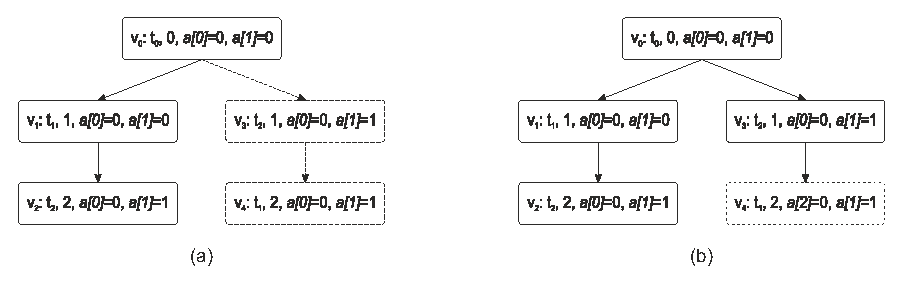
\includegraphics[width=14cm, height=4.0cm]{images/eps/Pereira_10_mpor.eps}
\caption{MPOR applied to a kernel with independent (Fig.~\ref{fig:kernelMpor}a) and dependent (Fig.~\ref{fig:kernelMpor}b) transitions.}
\label{fig:kernelMpor}
\end{figure*}

%-------------------------------------
\subsubsection{Differences from MPOR to other interleaving reduction methods}
\label{sec:Differencesfro MPOR}
%-------------------------------------	

There are software verifiers that apply interleaving reduction methods to CUDA program verification. As example, GKLEE implements a technique named as ``canonical scheduling'', which records all reads and writes that are run by each thread within barrier interval before continuing to the next thread. Records are related in pairs that can have conflicts and, by means of an SMT solver query, those conflicts are checked to detect whether data race condition exists. If conflicts are not detected, then the canonical schedule is defined to represent the barrier interval for the verification of other properties. The MPOR algorithm performs its analysis and reduction on verification time and checks the properties violation on-the-fly, by encoding (small) SMT formulae. GKLEE first checks data race condition to reduce schedules and then verifies other properties. We can observe that both approaches call several times its back-end verification engine, being GKLEE with canonical scheduling and ESBMC-GPU with BMC and Pthread using MPOR.

%-------------------------------------
\subsection{Two-threads Analysis}
\vspace{-2pt}
\label{sec:twothreadsReduction}
%-------------------------------------	

GPU architectures are composed by multiprocessors built upon \textbf{P}rocessing \textbf{E}lements (PE) sets~\cite{cuda:2012,cudaproguide:2015}.\ Those PEs are typically arranged in subgroups (named as warps), which run in the same lockstep, ensuring that threads inside those PEs can synchronize using barriers, while threads from one subgroup run independently~\cite{betts:2012} to threads from another subgroup. 

Similar to GPUVerify~\cite{betts:2012} (for checking race- and divergence-freedom) and PUG~\cite{Li:2010}, we also reduce the CUDA program verification to two threads for improving verification time and avoiding the state-space explosion problem. Since CUDA kernels typically manipulate one element of the array, and for each element one thread is used, the two-threads analysis ensures that, errors ({\it e.g.}, data races) that are detected between two threads in a given subgroup, due to unsynchronized accesses to shared variables, are enough to justify the property violation in the program.

   \begin{figure}[!htp]
   \centering
    \subfloat[NVIDIA Fermi GPU\label{subfig-1:fermi}]{%
      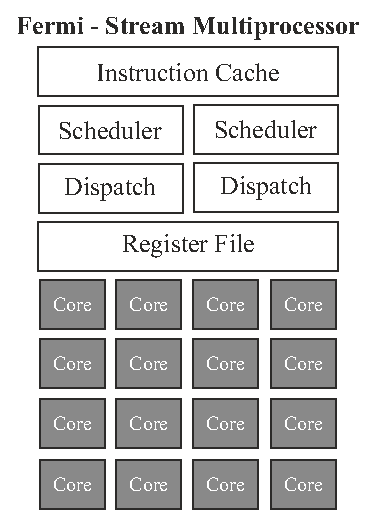
\includegraphics[width=0.29\textwidth]{images/eps/fermi-architecture-gray.eps}
    }
    \hspace{2em}
    \subfloat[Two-threads approach\label{subfig-2:two-thread}]{%
      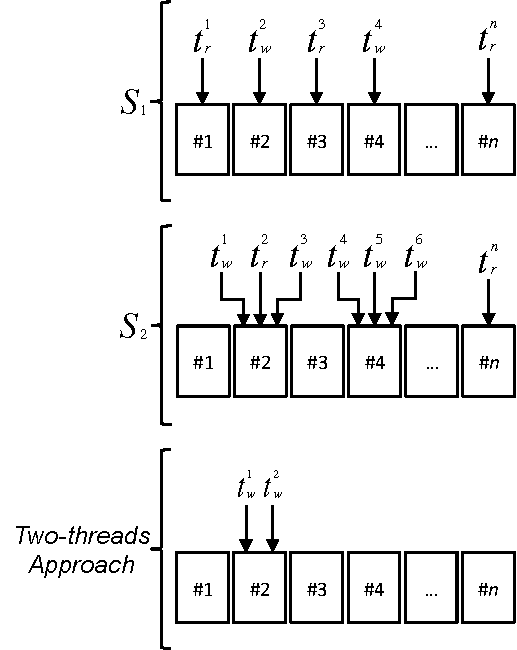
\includegraphics[width=0.39\textwidth]{images/two-thread-approach.pdf}
    }
    \caption{Comparison between the NVIDIA Fermi GPU architecture and the two-threads approach used by used to handle data.}
    \label{fig:comparison}
  \end{figure}
  
In order to demonstrate the reasoning upon two-threads analysis, a NVIDIA Fermi GPU~\cite{cudaproguide:2015} composed by $32$ processing cores is shown in Figure~\ref{fig:comparison}. Importantly, Figure~\ref{subfig-1:fermi} shows the architecture model of that GPU with $16$ processing cores (highlighted in grey boxes), because the thread processing is performed in half-warps~\cite{fermi:2009}, {\it i.e.}, $16$ threads of the same warp are scheduled, ensuring synchronization when a barrier occurs. Figure~\ref{subfig-2:two-thread} demonstrates the thread representation, which accesses the GPU shared memory. First of all, the numbered white boxes represent the shared memory positions to be accessed, ${t_{r}}^n$ are the thread-readers, and ${t_{w}}^n$ are the thread-writers, where $n$ is the index of each thread; it is worth noticed that the threads are executed on a streaming multiprocessor. In the first case of Figure~\ref{subfig-2:two-thread} (\textit{i.e.}, $S_{1}$), the threads, whose kernel is correctly implemented, do not present a data race condition, once they access different memory positions. In the second case of Figure~\ref{subfig-2:two-thread} (\textit{i.e.}, $S_{2}$), the threads execution of a kernel results in a data race condition, where several threads read or write in the same memory position, at the same lock-step. Finally, the third case of Figure~\ref{subfig-2:two-thread} is quite similar to the situation occurred in $S_{2}$, however, instead of using multiple threads to analyse data-race conditions, ESBMC-GPU ensures that such errors can be detected through the analysis of the behaviour of two threads that are operating over the same memory location.

Note that the two-threads analysis affects mostly the data race verification, where program states must be analyzed with respect to their possible threads interleavings, which lead to an execution order of statements that results in error. In our benchmarks, we observed a substantial performance improvement, considering only two threads, while keeping true incorrect results at low rates.

%---------------------------------------
\vspace{-6pt}
\section{Experimental Evaluation}
\vspace{-2pt}
\label{sec:resultadosExperimentais}
%---------------------------------------

%---------------------------------------
\subsection{Experimental Setup}
\vspace{-2pt}
\label{sec:PlanejamentoeDesenvolvimento}
%---------------------------------------

This section describes the experiments to investigate ESBMC-GPU performance for verifying CUDA programs.\
We also compare ESBMC-GPU to GKLEE~\cite{Li:2012}, GPUVerify~\cite{betts:2012}, PUG~\cite{Li:2010}, and CIVL~\cite{civl:2015}.\ In particular, we evaluate ESBMC-GPU's ability to verify $154$ benchmarks\footnote{ESBMC-GPU and benchmarks are available at http://esbmc-gpu.org}, which are extracted from~\cite{cuda:2012,betts:2012,cudaproguide:2015}; we added a \textit{main} function to those benchmarks that do not contain it. The kernels typically exploit the support for:  arithmetic operations, pointer assignment, $\_\_device\_\_$ function calls, general ANSI-C functions ({\it e.g.}, \textit{memset}, \textit{assert}), general CUDA functions ({\it e.g.}, \textit{atomicAdd}, \textit{cudaMemcpy}, \textit{cudaMalloc}, \textit{cudaFree}, \textit{\_\_syncthreads}), general libraries in CUDA ({\it e.g.}, \textit{curand.h}, \textit{curand\_kernel.h}, \textit{curand\_mtgp32\_host.h}) and the ability to work with variables \textit{int}, \textit{float}, \textit{char} as well as type modifiers ({\it e.g.}, \textit{long} and \textit{unsigned}), pointers to that variables, function pointers, type definitions, and intrinsic CUDA variables ({\it e.g.}, \textit{uint4}). 

Note that we used benchmarks from a variety of sources to evaluate ESBMC-GPU's precision and performance, which include CUDA benchmarks suite to check basic functions that are commonly used by real CUDA applications. Our benchmarks suite comprises of $20$ CUDA kernels from NVIDIA GPU Computing SDK v$2$.$0$~\cite{toolkit:2015}, $20$ CUDA kernels from Microsoft C$++$ AMP Sample Projects~\cite{microsoft:2012}, and $104$ CUDA programs that explore a wide range of CUDA functionalities~\cite{cuda:2012,cudaproguide:2015}. Although there are some CUDA benchmarks that do not implement real CUDA applications, they are still valuable to analyze to which extent ESBMC-GPU is able to handle and detect (known) errors; in particular, those benchmarks have been previously used for comparing the performance and precision of different GPU verifiers~\cite{betts:2012}. It is worth notice that the benchmarks related to OpenCL~\cite{Khronos:2011} were not applied to our experimental evaluation, once ESBMC-GPU does not support it yet.

Our experiments answer two research questions: RQ1 (sanity check) which results does ESBMC-GPU obtain upon verifying benchmarks that compose the specified suite? RQ2 (comparison with other tools) what is ESBMC-GPU performance when compared to GKLEE, GPUVerify, PUG, and CIVL?

To answer RQ1, ESBMC-GPU is executed with: \emph{\tt --force-malloc-success}, which considers that there is always enough memory available in the device; \emph{\tt --context-switch C}\footnote{The value of C ranges from $2$ to $4$ context switches.}, which considers a context-switch bound among all threads; and \emph{\tt --I libraries}, which specifies the library directory. We also replace the kernel call by the respective \textit{ESBMC\_verify\_kernel} function using one block and two threads per block. As example, we call ESBMC-GPU as: \emph{\tt esbmc file.cu} \emph{\tt --force-malloc-success --context-switch 2 --I libraries}.

To answer RQ2, we apply GKLEE, GPUVerify, PUG, and CIVL to the ESBMC-GPU benchmarks suite. With GKLEE, we use two commands: \textit{gklee-nvcc} and \textit{gklee}. The first one checks the file to be verified, with the extension ``.cu''. When this command is executed, two new files are generated: a ``.cpp'' file and a runnable file (without extension). Then, the second command is used with the generated runnable file. We call GKLEE as: \emph{\tt gklee-nvcc file.cu -libc=uclibc} or \emph{\tt gklee-nvcc file.cu -libc=klee; gklee file}.

To the verification of GPUVerify, the following modifications are required: 
(a) remove the main function; 
(b) check if the variable initialization performed by the main function is responsible for controlling some conditional declaration inside the kernel; if so, such variable must be initialized by \emph{\tt \_\_requires()} function; 
(c) check if there is any assertion in the kernel; if so, this assertion must be replaced by \emph{\tt \_\_assert()}; 
(d) check if there are specific functions to C/C$++$ libraries; if so, they must be removed, as they are not supported by GPUVerify. 
To run GPUVerify, two options must be used: \emph{\tt --gridDim=M} and \emph{\tt --blockDim=N} to assign the number of blocks and threads (per block), respectively. We call GPUVerify as: \emph{\tt gpuverify file.cu} \emph{\tt --blockDim=2 --gridDim=1}. 

Additional options for ESBMC-GPU and GPUVerify are necessary to check for data races and array out-of-bounds, respectively.

Some additional changes to the benchmarks are necessary to use PUG: 
(a) the file extension is changed from ``.cu'' to ``.c''; 
(b) given that PUG is unable to verify main functions, these must be removed, in order to keep the kernel function only; 
(c) PUG's proprietary libraries \textit{my\_cutil.h} and \textit{config.h} must be called inside the ``.c'' file. The first library has definitions of structs, qualifiers, and datatypes. The second one defines the number of blocks and threads (per block); 
(d) The kernel function's name has to be renamed to ``kernel''. As example, we call PUG as: \emph{\tt pug kernel.c}.

To verify CUDA programs with CIVL, we use the command \emph{\tt civl verify file.cu}. If the benchmark contains the \textit{malloc} and \textit{free} functions, we must manually add the standard ANSI-C library \textit{stdlib.h} to the CUDA program, although it is not mandatory to declare it according to the CUDA documentation~\cite{cuda:2012}.

All experiments were conducted on an otherwise idle Intel Core i$7$-$4790$ CPU $3$.$60$ GHz, $16$ GB of RAM, and Linux OS.\ All times given are wall clock time in seconds as measured by the UNIX time command.

%---------------------------------
\subsection{Evaluating SMT Solvers for Verifying CUDA Programs}
\vspace{-2pt}
%---------------------------------

ESBMC-GPU now supports five different SMT solvers: Z$3$ v$4$.$0$~\cite{Moura:2008}, Boolector v$2$.$0$.$1$~\cite{Brummayer:2009}, Yices v$2$.$3$.$1$~\cite{Dutertre:2014}, MathSAT v$5$~\cite{Cimatti:2013}, and CVC4~\cite{Deters:2014}. The flag $--$solver (\textit{e.g.},$--$boolector) is used to define an SMT solver, which is different from the standard ESBMC-GPU configuration. 

The solvers' performance is shown in Table~\ref{table:solvers}, where the 
``tool'' column describes the tool name, 
``true correct'' shows the result in which no error has been found for bug-free benchmarks,
``false correct'' shows the results in which the tool correctly detected a bug,
``true incorrect'' shows the results in which the tool did not detect a bug,
``false incorrect'' shows the results in which the tool incorrectly detected a bug,
``not supported'' shows the results which are not supported by the respective tool,
and ``time'' shows the total verification time.

Table~\ref{table:solvers} shows that Z$3$, Boolector, Yices, and MathSAT produce exactly the same number of true correct results (56). Additionally, Z3, Boolector, and Yices present $63$ false correct results, while MathSAT produced only $61$. These results ensure that Z3, Boolector, and Yices are the most effective SMT solvers for verifying CUDA programs in ESBMC-GPU, where correctness is an important parameter for evaluating the solvers performance. Additionally, if we consider verification time, then Z$3$ has an improved performance of $3,6\%$ over Yices. Thus, we defined Z3 as the (default) SMT solver to verify CUDA programs in ESBMC-GPU.

%---------------------------------
\subsection{Experimental Results}
\vspace{-2pt}
%---------------------------------

Table~\ref{table:nonlin} shows the results of ESBMC-GPU v$1$.$25$, GKLEE (LLVM v$3$.$2$), GPUVerify $2$, PUG (ROSE v$0$.$9$) and CIVL v$1$.$6$; each row means: 
tool name (Tool); 
total number of benchmarks in which the program was analyzed to be free of errors (True Correct); 
total number of benchmarks in which the error in the program was found and an error path was reported (False Correct);
total number of benchmarks in which the program had an error, but the verifier did not find it (True Incorrect); 
total number of benchmarks in which an error is reported for a program that fulfills the specification (False Incorrect);
total number of benchmarks which are not supported (Not Supported); 
verification time, in seconds, for all benchmarks (Time).

ESBMC-GPU is able to correctly verify $82.5\%$ of the benchmarks, GKLEE $71.4\%$, GPUVerify $57.1\%$, PUG $35.1\%$ and CIVL $30.5\%$. Note that ESBMC-GPU produces $1$ true incorrect results, while GKLEE produces $14$, GPUVerify produces $9$, PUG produces $7$ and CIVL does not produce any true incorrect result.
With ESBMC-GPU, this result is due to a null pointer access.\
With GKLEE, errors are due to failure in detecting data race ($10$), unsuccessful detection of attempts to modify constant memory ($2$), incorrect detected assertion ($1$), and null pointer access ($2$).
GPUVerify does not detect data race ($7$), does not detect an array bounds violation ($1$), and does not detect an assertion violation ($1$).

PUG does not detect access to null pointer ($1$), data race ($4$), array bounds violation ($1$), and incorrect detected assertion ($1$). ESBMC-GPU generated $3$ false incorrect results, due to assertions included in the kernel, which should return true, but it fails ($2$), and the partial coverage of the \textit{cudaMalloc} function for copies of float-type variables ($1$).
GKLEE generated $7$ false incorrect results, which are caused by incorrectly detected assertions ($4$), data-races ($1$), array out-of-bounds ($1$) and solver call failure ($1$).
GPUVerify generated $8$ false incorrect results, due to incorrectly detected assertion ($2$) and data-races ($6$).
PUG produces $11$ false incorrect results due to data races incorrectly detected.
CIVL produces $3$ false incorrect results due to detection of memory allocation error ($2$) and assertions ($1$).

ESBMC-GPU had $23$ benchmarks that were not supported. These are related to constant memory access ($3$), the use of CUDA's specific libraries (\textit{e.g., curand.h}) ($7$), and the use of pointers to functions, structures, and char type variables used as kernel call arguments ($13$).
GKLEE has $22$ benchmarks that were not supported, which are due to incorrectly detected assertions ($2$); function pointers ($11$), either used as kernel arguments or as in any other parts of the CUDA program; specific CUDA libraries \textit{curand.h} ($7$), and \textit{switch-case} functions ($2$).

GPUVerify did not support $49$ benchmarks. Since it does not support main functions, this explains most cases ($39$); it also does not support the use of \textit{memset} function ($2$), the array bounds detection ($2$), the use of \textit{math\_functions} ($1$), while  other cases are explained by the absence of support to function pointers, either as kernel function arguments or as in any other part of the CUDA program ($5$).

PUG does not support $82$ benchmarks. As GPUVerify, PUG does not verify main functions and this explains most unsupported cases ($31$), while others are explained by the lack of support to \textit{\_\_syncthreads} function ($12$), function pointers ($9$), and the \textit{curand.h} library ($7$); additionally, PUG does not support the use of unsigned type modifier as argument to the function \textit{atomicAdd} ($6$); changes in variables stored in constant memory ($3$), and inability to handle structs ($2$), variables with \textit{\_\_device\_\_} qualifier ($2$), and \textit{size\_t} type ($1$), in addition to other cases that PUG aborted by returning a false null pointer access ($7$) or because it did not recognize the NULL identifier ($2$).

CILV does not support $104$ benchmarks, this is caused by the use of \textit{atomic functions} ($18$), \textit{cudaThreadSynchronize} ($10$), \textit{threadIdx} ($10$), function \textit{typedef} ($8$), \textit{curand functions} ($7$), \textit{dim3} ($6$), \textit{math\_functions} ($5$), \textit{uint4} ($5$), \textit{\_\_constant\_\_ variables} ($5$), \textit{\_\_attribute\_\_} ($5$), \textit{\_\_restrict}  ($2$),  structs ($2$), scanf ($2$), boolean functions (e.g AND and OR) ($2$), \textit{uint} ($2$), \textit{extern} C ($1$), \textit{\_\_threadfence}  ($1$), typecast ($1$). Other benchmarks could not be verified due to the existence of data-race in benchmarks ($11$) and undefined cases ($1$).

%---------------------------------
\subsubsection{ESBMC-GPU effectiveness over existing GPU verifiers}
\vspace{-2pt}
%---------------------------------

MPOR produced an improved performance of approximately $80\%$ in our benchmarks; in particular, it reduced the verification time from $16$ to $3$ hours. With two-threads analysis, we further reduced the verification time from $3$ hours to $811$ seconds. Although the application of these techniques has considerably improved the ESBMC-GPU performance, it still takes more (verification) time than all other existing tools. This is due to the actual execution of the threads interleavings (which combines symbolic model checking with explicit state space exploration), while in GPUVerify the analysis is fully symbolic, performed only in the kernel level, without considering threads interleavings with the main thread. PUG lower verification time is due to the two-threads analysis and because it does not perform the \textit{main function} verification. GKLEE presents a low verification time due to its directed state/path reduction method.

Additionally, in order to improve the verification performance, ESBMC-GPU uses an abstract representation of the CUDA libraries that properly reflects their semantics. This abstract representation includes pre/post-conditions and simulation features that consider only relevant behavior to be explored from the verification perspective, {\it i.e.}, irrelevant code fragments that unnecessarily complicate the generated VCs are actually abstracted. As a result, during the ESBMC-GPU verification process, the COM replaces the real CUDA libraries, which thus improves its effectiveness to detect more properties violations than other existing GPU verifiers, as shown in our experimental evaluation.

%------------------------------
\vspace{-6pt}
\section{Conclusions}
\label{sec:conclusions}
\vspace{-2pt}
%------------------------------

ESBMC-GPU is able to verify CUDA programs using SMT-based context-bounded model checking and operational models, which recognize CUDA directives and further simplify the verification model.\ This work marks the first application of symbolic model checking with explicit state space exploration using MPOR for verifying CUDA programs. In particular, MPOR led to $80$\% of performance improvement in our benchmarks.\
ESBMC-GPU also presents an improved ability to detect array out-of-bounds and data race violations if compared to GKLEE, GPUVerify, PUG, and CIVL. Additionally, ESBMC-GPU provides fewer incorrect results than all other existing GPU verifiers.
Experimental results also show that ESBMC-GPU presents a successful verification rate of $82.5\%$, compared to $71.4\%$ of GKLEE, $57.1\%$ of GPUVerify, $35.1\%$ of PUG, and $30.5\%$ of CIVL. For future work, we will improve our support to argument types of kernel functions, support stream interleaving, and apply techniques to reduce the number of threads interleavings. Besides, conformance testing procedures will be developed for further validating COM, which could also be applied to CUDA modules.

\noindent \textbf{Acknowledgements.} This research project was supported by the Institute of Technology Development (INDT) and by CNPq 475647/2013-0 (UNIVERSAL).

% ---------------------------------------
\begin{thebibliography}{99}

%1
\bibitem{cuda:2012}
Cheng J, Grossman M, McKercher T.
\newblock {\em {Professional CUDA C Programming}}.
\newblock {John Wiley and Sons, Inc.} 2014.

%2
\bibitem{gpu:2010}
Kirk D, Hwu W.
\newblock {\em {Programming Massively Parallel Processors}}.
\newblock Elsevier Inc. 2010.

%3
\bibitem{betts:2012}
Betts A, Chong N, Donaldson AF, Qadeer S, Thomson P.
%A.~Betts {\it et al.}
\newblock {\em{GPUVerify: A Verifier for {GPU} Kernels}}.
\newblock {OOPSLA} 2012; 113--132.

%4
\bibitem{cordeiro:2011}
Cordeiro L, Fischer B.
\newblock {\em{Verifying Multi-threaded Software using SMT-based Context-Bounded
  Model Checking}}.
\newblock {ICSE} 2011; 331--340.

%5
\bibitem{cordeiro:2012}
Cordeiro L, Fischer B, Marques{-}Silva J.
\newblock {\em{SMT-Based Bounded Model Checking for Embedded {ANSI-C} Software}}.
\newblock {IEEE} Trans. Software Eng. 2012; 38(4):957--974.

%6
\bibitem{ramalho:2013}
%M.~Ramalho {\it et al.}
Ramalho M, Freitas M, Sousa F, Marques H, Cordeiro L, Fischer B.
\newblock {\em{SMT-Based Bounded Model Checking of C++ Programs}}.
\newblock {{ECBS}} 2013; 147--156.

%7
\bibitem{Li:2010}
Li G, Gopalakrishnan G.
\newblock {\em{Scalable SMT-based Verification of GPU Kernel Functions}}.
\newblock {FSE} 2010; 187--196.

%8
\bibitem{Li:2012}
%G.~Li {\it et al.}
Li G, Li P, Sawaya G, Gopalakrishnan G, Ghosh I, Rajan SP.
\newblock {\em{GKLEE: Concolic Verification and Test Generation for GPUs.}}
\newblock {PPoPP} 2012; 215--224.

%9
\bibitem{civl:2015}
%M.~Zheng {\it et al.}
Zheng M, Rogers M, Luo Z, Dwyer M, Siegel S.
\newblock {\em{{CIVL}: Formal Verification of Parallel Programs}}.
\newblock {ASE} 2015.

%10
\bibitem{Biere:2009}
A.~Biere.
\newblock {\em{Bounded Model Checking. Handbook of Satisfiability}}. 
\newblock {IOS Press} 2009; 457--481.

%11
\bibitem{Barrett:2009}
Barrett C, Sebastiani R, Seshia S, Tinelli C.
\newblock {\em{ Satisfiability Modulo Theories. Handbook of Satisfiability}}.
\newblock {IOS Press} 2009; 825--885.

%12
\bibitem{KahlonWG09}
Kahlon V, Wang C, Gupta A.
\newblock {\em{Monotonic Partial Order Reduction: An Optimal Symbolic Partial Order
  Reduction Technique}}.
\newblock {CAV} 2009; 398--413.

%13
\bibitem{cudaproguide:2015}
NVIDIA.
\newblock {\em {CUDA C Programming Guide}}.
\newblock NVIDIA Corporation 2015.


%14
\bibitem{Pereira15}
Pereira P, Albuquerque H, Marques H, Silva I, Carvalho C, Santos V, Ferreira R, Cordeiro L.
\newblock {\em{Verifica\c{c}\~ao de Kernels em Programas CUDA usando Bounded Model Checking.}} 
\newblock {WSCAD-SSC} 2015; 24--35.

%15
\bibitem{Pereira16}
Pereira P, Albuquerque H, Marques H, Silva I, Carvalho C, Santos V, Ferreira R, Cordeiro L.
\newblock {\em{Verifying CUDA Programs using SMT-Based Context-Bounded Model Checking.}} 
\newblock {SAC SVT track 2016; 1648--1653.}

%16
\bibitem{boogie:2011}
Le~Goues C, Leino KRM, Moskal M.
\newblock {\em{The Boogie Verification Debugger}.}
\newblock {{SEFM} 2011; 407--414.}

%17
\bibitem{Moura:2008}
Moura L, Bjorner N.
\newblock {\em {Z3: An Efficient SMT Solver}}. 
\newblock {TACAS} 2008; 337--340.

%18
\bibitem{CVC4Barrett11}
%C. ~Barrett {\it et al.}
Barrett C, Conway C, Deters M, Hadarean L, Jovanovi\'{c} D, King T, Reynolds A, Tinelli C.
\newblock {\em{CVC4.}}
\newblock   {CAV} 2011; 171--177.

%19
\bibitem{sesa:2014}
Li P, Li G, Gopalakrishnan G.
\newblock {\em{Practical Symbolic Race Checking of {GPU} Programs}}.
\newblock {SC} 2014; 179--190.

%20
\bibitem{Morse11}
Morse J, Cordeiro L, Nicole D, Fischer B.
\newblock {\em{Context-Bounded Model Checking of LTL Properties for ANSI-C Software.}} 
\newblock {SEFM} 2011; 302--317.

%21
\bibitem{Morse:15}
Morse J, Cordeiro L, Nicole D, Fischer B.
\newblock {\em{Model checking LTL properties over ANSI-C programs with bounded traces.}} 
\newblock {Software and System Modeling} 2015; 14(1): 65--81.

%22
\bibitem{svcomp2014}
Beyer, D.
\newblock{\em{Status report on software verification.}}
%\newblock In Tools and Algorithms for
%  the Construction and Analysis of Systems, LNCS, vol. 8413, pp. 373--388.
%  Springer Berlin Heidelberg (2014)
\newblock {TACAS} 2014; 373--388.
  
%23
\bibitem{svcomp2015}
Beyer, D.
\newblock{\em{Software verification and verifiable witnesses.}}
\newblock{TACAS} 2015; 401--416.

%24
\bibitem{Clarke:2004}
Clarke E, Kroening D, Lerda F.
\newblock {\em {A Tool for Checking ANSI-C Programs}}.
\newblock {TACAS} 2004; 168--176.

%25
\bibitem{Levine:2009:FB:1696439}
Levine J, John L.
\newblock {\em {Flex \& Bison}}.
\newblock 1st Edition, O'Reilly Media, Inc., 2009.

%26
\bibitem{Lopes:2014:GSL:2692607}
Lopes B, Auler R 
\newblock {\em {Getting Started with LLVM Core Libraries}}. 
\newblock Packt Publishing, 2014.

%27
\bibitem{clang-usage}
M.~Cade. 
\newblock {\em {Why {A}pple’s swift language will instantly remake computer programming}}.
\newblock http://www.wired.com/2014/07/apple-swift/, 2016.

%28
\bibitem{cytron89}
Cytron R, Ferrante J, Rosen B, Wegman M, Zadeck F. 
\newblock {\em {An Efficient Method of Computing Static Single Assignment Form}}
\newblock {POPL} 1989; 25--35.

%29
\bibitem{monteiro:2015}
Monteiro F, Cordeiro L, de Lima Filho E. 
\newblock {\em {Bounded Model Checking of C++ Programs Based on the Qt Framework}}. 
\newblock {GCCE} 2015; 179--447.
%\newblock {DOI=http://dx.doi.org/10.1109/GCCE.2015.7398699}}

%30
\bibitem{garcia:2016}
Garcia M, Monteiro F, Cordeiro L, de Lima Filho E. 
\newblock {\em {ESBMC$^{QtOM}$: A Bounded Model Checking Tool to Verify Qt Applications}}. 
\newblock {SPIN} 2016; 97--103.
%\newblock {DOI=http://dx.doi.org/10.1007/978-3-319-32582-8\_6}}

%31
\bibitem{android:2012}
Heila van der Merwe, Brink van der Merwe, and Willem Visser.
\newblock {\em {Verifying android applications using Java PathFinder}}
\newblock {SIGSOFT Softw. Eng. Notes 37, 6} 2012; 1-5.
%\newblock {DOI=http://dx.doi.org/10.1145/2382756.2382797}}

%32
\bibitem{android:2015}
Heila van der Merwe, Oksana Tkachuk, Brink van der Merwe, and Willem Visser.
\newblock {\em {Generation of Library Models for Verification of Android Applications}}
\newblock {SIGSOFT Softw. Eng. Notes 40, 1} 2015; 1-5.
%\newblock {DOI=http://dx.doi.org/10.1145/2693208.2693247}}

%33
\bibitem{tacas14}
Morse J, Ramalho M, Cordeiro L, Nicole D, Fischer B.
\newblock ESBMC 1.22 - (Competition Contribution).
\newblock {TACAS} 2014; 405--407.

%34
\bibitem{Mehtaa:2005}
Mehtaa F, Nipkowb T.
\newblock {\em {Proving pointer programs in higher-order logic}}.
\newblock {Information and Computation} 2005; 199(1), 200--227.

%35
\bibitem{Pedro:2011}
C\'amara P, Castro J, Gallardo M, Merino P.
\newblock {\em {Verification support for ARINC-653-based avionics software}}.
\newblock {JSTVR} 2011; 21(4): 267--298.

%36
\bibitem{Pedro:2009}
C\'amara P, Gallardo M, Merino P, San\'an D.
\newblock {\em {Checking the reliability of socket based communication software}}. 
\newblock {STTT} 2009; 11(5): 359-374.

%37
\bibitem{morse:2015}
Morse J.
\newblock {\em {Expressive and Efficient Bounded Model Checking of Concurrent Software}}.
\newblock {University of Southampton, PhD Thesis} 2015.

%38
\bibitem{posix:2008}
Institute of Electrical and Electronics Engineers, Inc.
\newblock {\em {IEEE Standard for Information Technology - Portable Operating System Interface (POSIX) Base Specifications, IEEE Std 1003.1-2008 (Revision of IEEE Std 1003.1-2004)}}.
\newblock {IEEE} 2008.

%39
\bibitem{fermi:2009}
NVIDIA.
\newblock {\em {CUDA Compute Architecture: Fermi}}.
\newblock {NVIDIA Corporation} 2009.

%40
\bibitem{Brummayer:2009}
Brummayer R, Biere A.
\newblock {\em {Boolector: An Efficient SMT Solver for Bit-Vectors and Arrays}}. 
\newblock {TACAS} 2009; 174--177.

%41
\bibitem{Dutertre:2014}
B.~Dutertre.
\newblock {\em {Yices 2.2}}. 
\newblock {CAV} 2014; 737--744.

%42
\bibitem{Cimatti:2013}
Cimatti A, Griggio A, Schaafsma B, Sebastiani R.
\newblock {\em {The MathSAT5 SMT Solver}}.
\newblock {TACAS} 2013; 93--107.

%43
\bibitem{Deters:2014}
Deters M, Reynolds A, King T, Barrett C, Tinelli C.
\newblock {\em {A tour of CVC4: How it works, and how to use it}}. 
\newblock {FMCAD} 2014; 7.

%44
\bibitem{toolkit:2015}
NVIDIA.
\newblock {\em {CUDA Toolkit Release Archive}}. 
\newblock url{https://developer.nvidia.com/cuda-toolkit-archive}, 2015.

%45
\bibitem{microsoft:2012}
Microsoft Corporation.
\newblock {\em {C++ AMP sample projects for download (MSDN blog)}}. 
\newblock url{blogs.msdn.com/b/nativeconcurrency/archive/2012/01/30/c-amp-sample-projects-for-download.aspx}, 2012.

%46
\bibitem{Khronos:2011}
Khronos OpenCL Working Group.
\newblock {\em {The OpenCL Specification - version 1.1}}. 
\newblock Document Revision: 44, 2011.
\end{thebibliography}

\newpage

\begin{table*}[bh]
 \caption{Results of the SMT Solvers Performance. \textbf{True Correct} represents the number of flawless benchmarks correctly verified, while \textbf{True Incorrect} represents the ones verified incorrectly. Similarly, \textbf{False Correct} represents the number of faulty benchmark verified correctly, while \textbf{False Incorrect} represents the ones verified incorrectly. Not Supported represents the number of benchmarks unsuccessfully verified, \textbf{Time} represents the total verification time for each solver, and bold numbers represent the best results in each category.}
\centering
\label{table:solvers}
\begin{tabular}{c c c c c c c}
\hline
\multicolumn{1}{|l|}{\textbf{Result/Tool}}
& \multicolumn{1}{c|}{\textbf{Z3 4.0}} & \multicolumn{1}{c|}{\textbf{Boolector 2.0.1}} & \multicolumn{1}{c|}{\textbf{Yices 2.3.1}}
& \multicolumn{1}{c|}{\textbf{CVC 4}} & \multicolumn{1}{c|}{\textbf{MathSAT 5}} \\ \hline
\multicolumn{1}{|l|}{True Correct}
& \multicolumn{1}{c|}{\textbf{56}} & \multicolumn{1}{c|}{\textbf{56}} 
& \multicolumn{1}{c|}{\textbf{56}} & \multicolumn{1}{c|}{35} & \multicolumn{1}{c|}{\textbf{56}} \\ \hline

\multicolumn{1}{|l|}{False Correct}
& \multicolumn{1}{c|}{\textbf{63}} & \multicolumn{1}{c|}{\textbf{63}} 
& \multicolumn{1}{c|}{\textbf{63}} & \multicolumn{1}{c|}{60} & \multicolumn{1}{c|}{61} \\ \hline

\multicolumn{1}{|l|}{True Incorrect}
& \multicolumn{1}{c|}{\textbf{2}} & \multicolumn{1}{c|}{\textbf{2}} 
& \multicolumn{1}{c|}{\textbf{\textbf{2}}} & \multicolumn{1}{c|}{4} & \multicolumn{1}{c|}{\textbf{2}} \\ \hline

\multicolumn{1}{|l|}{False Incorrect}
& \multicolumn{1}{c|}{5} & \multicolumn{1}{c|}{5} 
& \multicolumn{1}{c|}{4} & \multicolumn{1}{c|}{28} & \multicolumn{1}{c|}{\textbf{2}} \\ \hline

\multicolumn{1}{|l|}{Not supported}
& \multicolumn{1}{c|}{28} & \multicolumn{1}{c|}{28} 
& \multicolumn{1}{c|}{29} & \multicolumn{1}{c|}{\textbf{27}} & \multicolumn{1}{c|}{33} \\ \hline

\multicolumn{1}{|l|}{\textbf{Time (s)}}
& \multicolumn{1}{c|}{\textbf{1828}} & \multicolumn{1}{c|}{4614} 
& \multicolumn{1}{c|}{1894} & \multicolumn{1}{c|}{3326} & \multicolumn{1}{c|}{8398} \\ \hline
\end{tabular}
\end{table*}

\newpage
\begin{table*}[bh]
 \caption{Results of ESBMC-GPU, GKLEE, GPUVerify, PUG, and CIVL. \textbf{True Correct} represents the number of flawless benchmarks correctly verified, while \textbf{True Incorrect} represents the ones verified incorrectly. Similarly, \textbf{False Correct} represents the number of faulty benchmarks verified correctly, while \textbf{False Incorrect} represents the ones verified incorrectly. \textbf{Not Supported} represents the number of benchmarks unsuccessfully verified, \textbf{Time} represents the total verification time for each verifier, and bold numbers represent the best results in each category.}
\centering
\label{table:nonlin}
\begin{tabular}{c c c c c c c}
\hline
\multicolumn{2}{|c|}{\textbf{Result/Tool}}
& \multicolumn{1}{c|}{\textbf{ESBMC-GPU}}	& \multicolumn{1}{c|}{\textbf{GKLEE}}	& \multicolumn{1}{c|}{\textbf{GPUVerify}}	& \multicolumn{1}{c|}{\textbf{PUG}}	& \multicolumn{1}{c|}{\textbf{CIVL}}	\\ \hline
\multicolumn{2}{|c|}{True Correct}
& \multicolumn{1}{c|}{\textbf{60}}		& \multicolumn{1}{c|}{53}	& \multicolumn{1}{c|}{58}	& \multicolumn{1}{c|}{39}	& \multicolumn{1}{c|}{23}	\\ \hline
\multicolumn{2}{|c|}{False Correct}                                               
& \multicolumn{1}{c|}{\textbf{67}} 		& \multicolumn{1}{c|}{57}	& \multicolumn{1}{c|}{30} 	& \multicolumn{1}{c|}{15}	& \multicolumn{1}{c|}{24}	\\ \hline
\multicolumn{2}{|c|}{True Incorrect}
& \multicolumn{1}{c|}{1}			& \multicolumn{1}{c|}{14}       & \multicolumn{1}{c|}{9}	& \multicolumn{1}{c|}{7}	& \multicolumn{1}{c|}{\textbf{0}}	\\ \hline
\multicolumn{2}{|c|}{False Incorrect}
& \multicolumn{1}{c|}{\textbf{3}}		& \multicolumn{1}{c|}{8}        & \multicolumn{1}{c|}{8}	& \multicolumn{1}{c|}{11}	& \multicolumn{1}{c|}{\textbf{3}}	\\ \hline
\multicolumn{2}{|c|}{Not Supported}
& \multicolumn{1}{c|}{23}		& \multicolumn{1}{c|}{\textbf{22}}       & \multicolumn{1}{c|}{49}	& \multicolumn{1}{c|}{82}	& \multicolumn{1}{c|}{104}	\\ \hline
\multicolumn{2}{|c|}{\textbf{Time (s)}}
& \multicolumn{1}{c|}{811}			& \multicolumn{1}{c|}{128}	& \multicolumn{1}{c|}{147}     	& \multicolumn{1}{c|}{\textbf{12}} & \multicolumn{1}{c|}{158}	\\ \hline
\end{tabular}
\end{table*}

\end{document}
